% Editable vector version of distance-1.png.
% Regenerate from this directory:
% latex -interaction=nonstopmode -halt-on-error distance-1.tex
% dvisvgm --no-fonts --exact --bbox=papersize --output=distance-1.svg distance-1.dvi
\documentclass[tikz,border=0pt]{standalone}
\usepackage[T1]{fontenc}
\usepackage{lmodern}
\definecolor{pathred}{RGB}{214,84,84}
\definecolor{pathblue}{RGB}{75,135,197}
\definecolor{pathgreen}{RGB}{100,162,107}
\definecolor{pathorange}{RGB}{229,140,81}
\definecolor{pathyellow}{RGB}{255,223,64}
\definecolor{pointblue}{RGB}{21,101,192}
\begin{document}
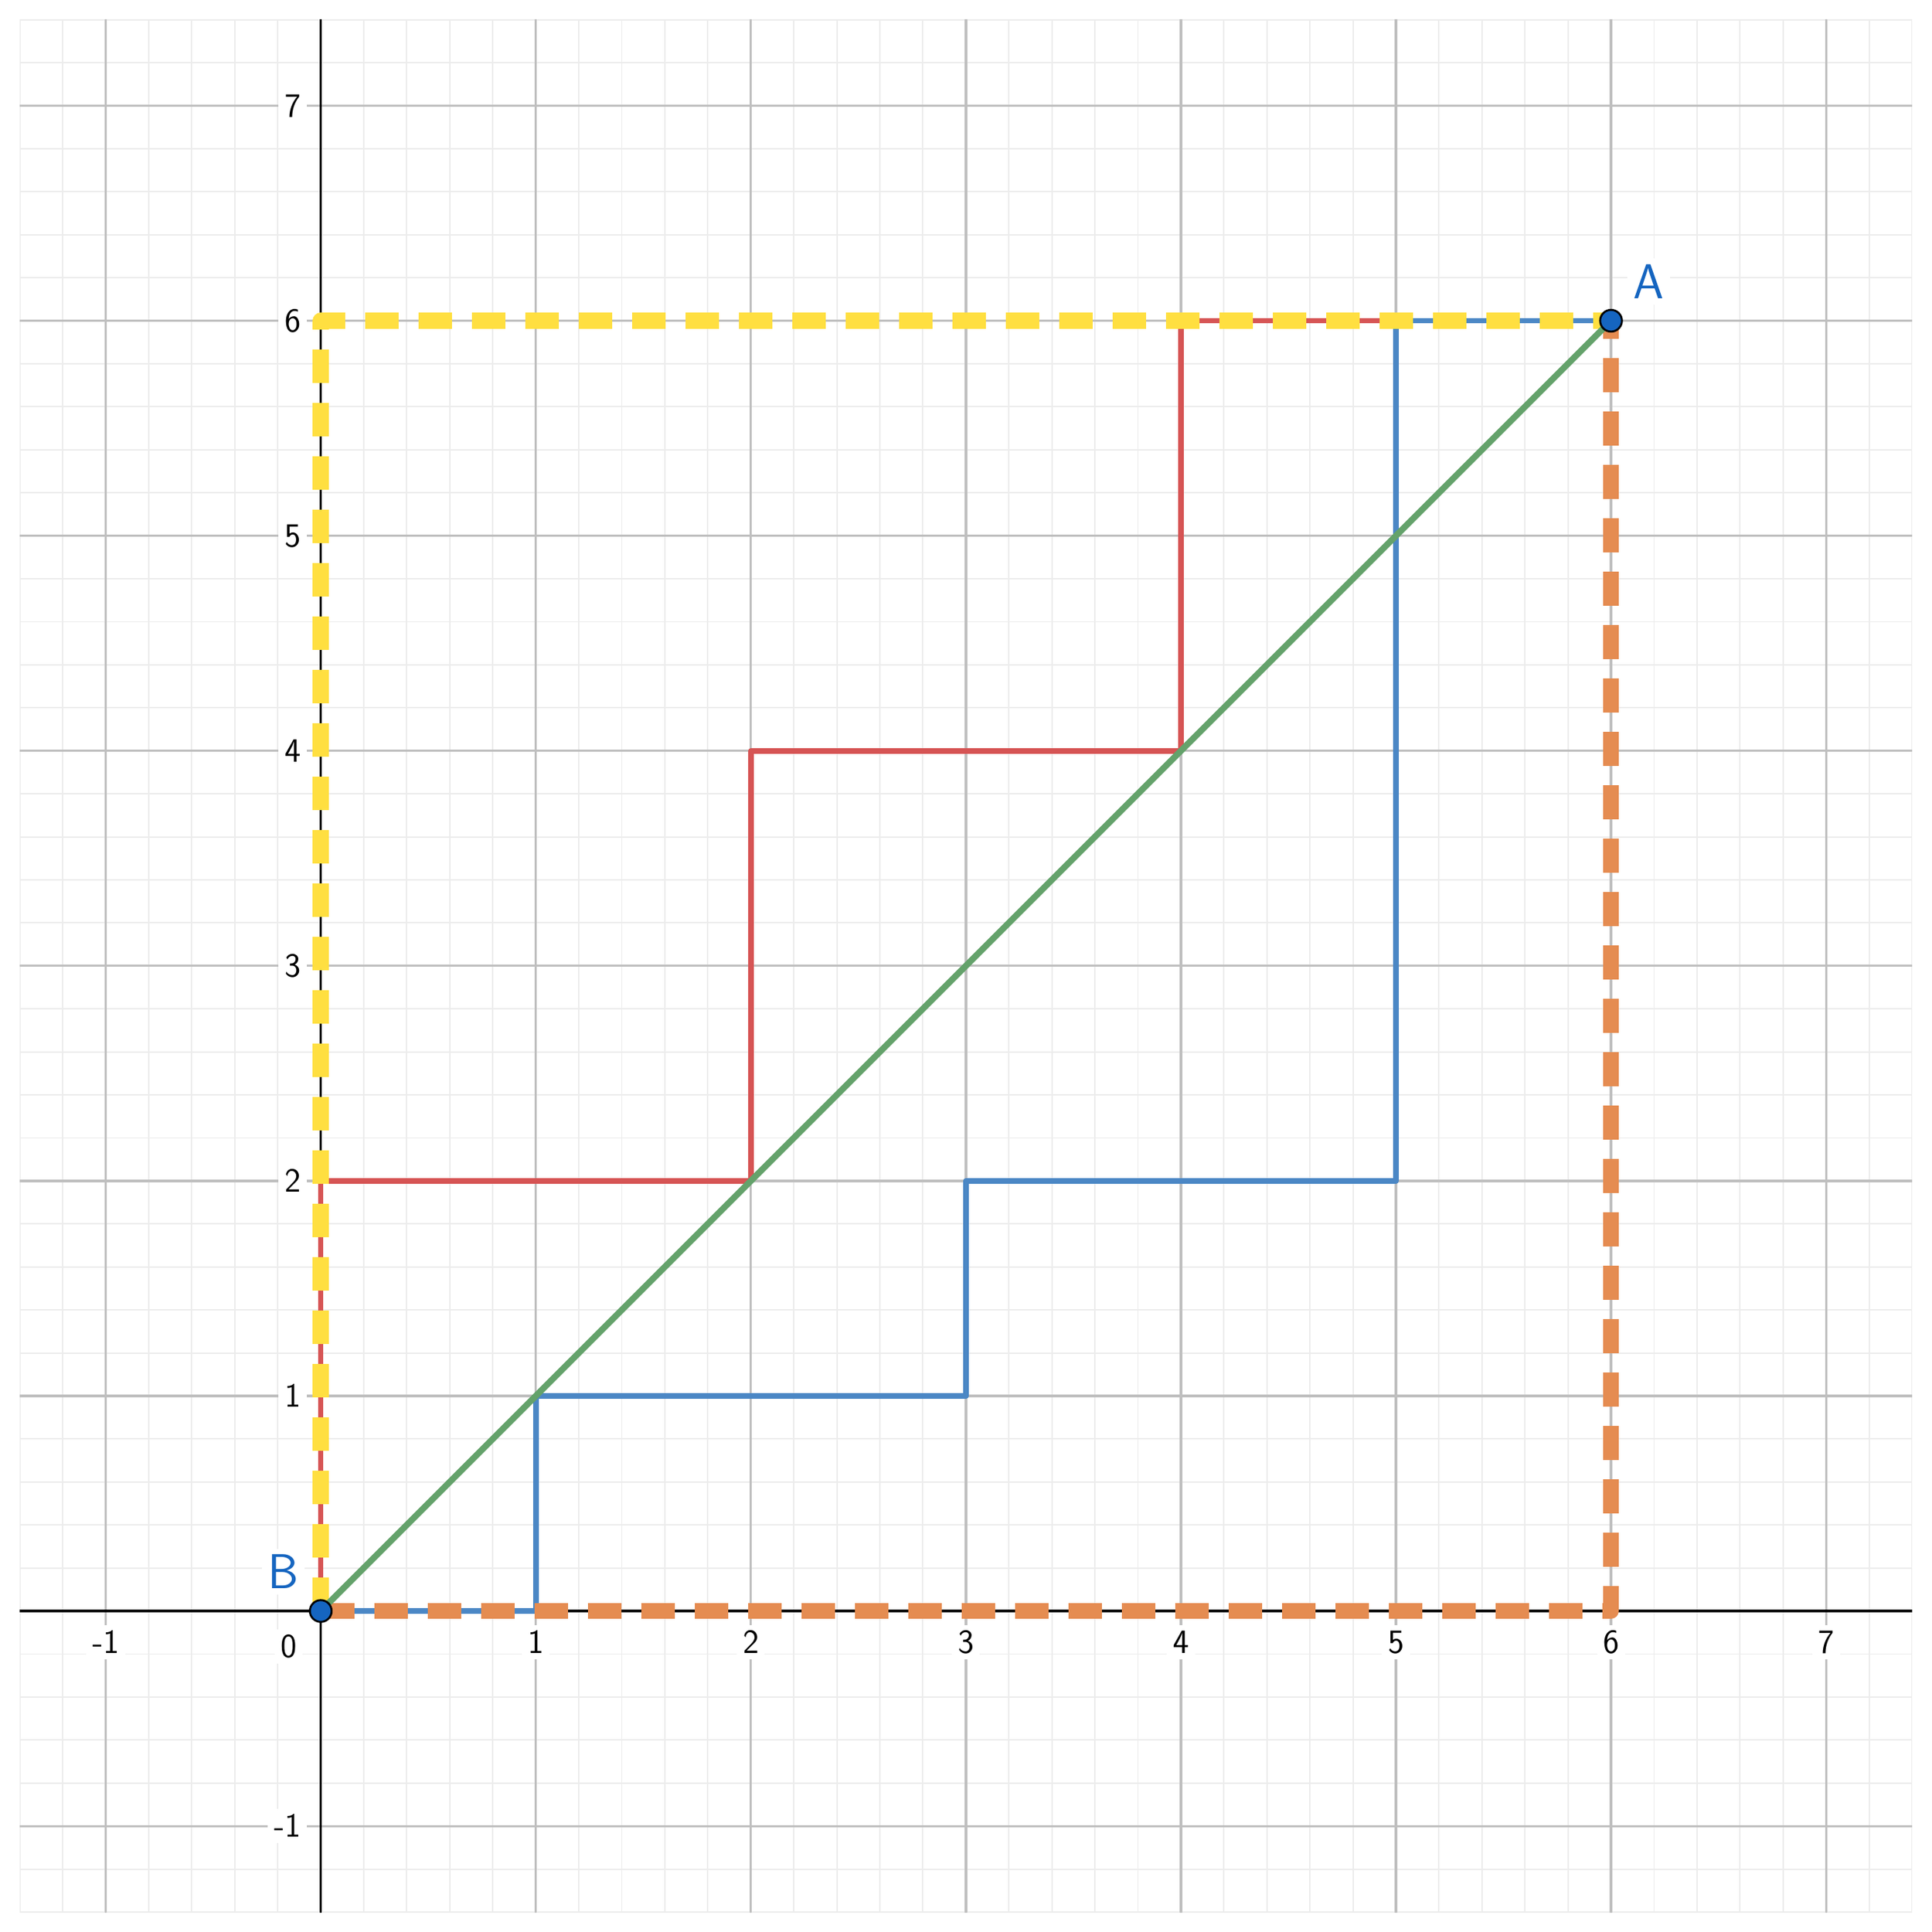
\begin{tikzpicture}[x=108.75bp,y=108.75bp,
  line cap=round,line join=round,
  every node/.style={fill=white,inner sep=3bp,
    font=\sffamily\fontsize{18bp}{21bp}\selectfont}]
  \path[use as bounding box] (-1.4,-1.4) rectangle (7.4,7.4);
  \clip (-1.4,-1.4) rectangle (7.4,7.4);
  \fill[white] (-1.4,-1.4) rectangle (7.4,7.4);
  \draw[step=0.2,gray!15,line width=0.7bp] (-1.4,-1.4) grid (7.4,7.4);
  \draw[step=1,gray!50,line width=1.2bp] (-1.4,-1.4) grid (7.4,7.4);
  \draw[line width=1.2bp] (-1.4,0) -- (7.4,0) (0,-1.4) -- (0,7.4);
  \coordinate (B) at (0,0);
  \coordinate (A) at (6,6);
  % Each axis-aligned path is monotone and has total length 6 + 6 = 12.
  \draw[pathred,line width=2.8bp] (B) -- (0,2) -- (2,2) -- (2,4)
    -- (4,4) -- (4,6) -- (A);
  \draw[pathblue,line width=2.8bp] (B) -- (1,0) -- (1,1) -- (3,1)
    -- (3,2) -- (5,2) -- (5,6) -- (A);
  \draw[pathyellow,line width=8bp,line cap=butt,dash pattern=on 17bp off 10bp]
    (B) -- (0,6) -- (A);
  \draw[pathorange,line width=8bp,line cap=butt,dash pattern=on 17bp off 10bp]
    (B) -- (6,0) -- (A);
  % The straight segment instead has Euclidean length 6 sqrt(2).
  \draw[pathgreen,line width=3.2bp] (B) -- (A);
  \foreach \point in {A,B} {
    \filldraw[fill=pointblue,draw=black,line width=1bp]
      (\point) circle[radius=5.5bp];
  }

  % Keep all text in the foreground and clear the grid beneath each label.
  \foreach \value in {-1,1,2,3,4,5,6,7} {
    \node[below=7bp] at (\value,0) {\value};
    \node[left=7bp] at (0,\value) {\value};
  }
  \node[below left=9bp] at (0,0) {0};
  \node[text=pointblue,above right=8bp,
    font=\sffamily\fontsize{24bp}{28bp}\selectfont] at (A) {A};
  \node[text=pointblue,above left=8bp,
    font=\sffamily\fontsize{24bp}{28bp}\selectfont] at (B) {B};
\end{tikzpicture}
\end{document}
